\chapter{Superconductivity and quench: an overview}
\label{chp:soupcond-quench}
In this chapter I will explain the very basic concepts of superconductivity and
superconductor quench applied to the field of superconducting magnets for particle accelerators.
\section{Superconductivity in theory}
\label{sec:soupcond}
Electronic motion in metallic or insulating materials is a very well studied and documented
phenomenon. Electrons passing through any material, endure a varying amount of disturbance based on
the type and structure of the material, this disturbance is known as electrical resistivity $\rho$. Given a
sample of a material of length $l$, cross-section $A$ and electrical resistance $R$, which is a
measure of its opposition to the flow of electric current, electrical resistivity can be computed
as:
\begin{equation}
	\label{eq:resistivity-cable}
	\rho = \frac{RA}{l} = \frac{m}{ne^2\tau}
\end{equation}
As highlighted in the second part of the equation, the resistivity of a material can be seen as a function of:
\begin{itemize}
	\item The mass of the electron $m$,
	\item The charge density $n$ of the material lattice,
	\item The charge of the electron $e$,
	\item The \emph{relaxation time} of the electron, which is the time interval occurring between two
	      successive electronic collisions $\tau$.
\end{itemize}
This other formulation allows us to interpret the resistivity based on the amount of electronic
interactions registered within the sample. The higher the number of interactions, the lower the
relaxation time, the higher the resistivity of the material.

Based on their value of resistivity, materials can be divided between metals and insulators. Metals
have a very low value of resistivity (usually less than $10^{-5}\Omega\cdot m$), while insulators impede the
flow of electric current. The resistivity for any sample of material can be described also as a
function of the temperature, if we suppose that its resistivity was measured at a reference
temperature $T_0$ and one is interested in the resistivity at a certain temperature $T$, it's
possible to link the resistivity at temperature $T$, $\rho_T$, to the reference resistivity,
$\rho_0$ and the temperature change $T - T_0$ multiplied by a regularization term.
\begin{equation}
	\label{eq:resistivity-func-of-temp}
	\rho_T = \rho_0[1 + \alpha(T - T_0)]
\end{equation}
$\alpha$ is known as the temperature coefficient of resistance, which is commonly defined as the
change in electrical resistance per degree of temperature change. Usually, pure metals have a
positive value of $\alpha$: copper, for instance, has $\alpha \approx 0.004\C^{-1})$; alloys can be
created to have coefficients close to $0\C^{-1}$. As a general rule of thumb, whenever the
temperature increases the resistivity of a metal increases, this is not necessarily
true for insulators. Thermal breakdown for insulators is a similar phenomenon to electrical
breakdown (the voltage reaches a critical level and the dielectric behaves like a normal conductor,
whenever we see a lightning we are experiencing electrical insulator breakdown, where the insulator
is air), if the temperature is too high the insulator breaks down and behaves like a normal conductor. A thorough description of the phenomenon is given in~\cite{kuvyrkin2022}

Superconductors are metals that follow classical thermodynamic properties when the temperature is
kept around ambient temperature. Their properties change drastically once the temperature gets
extremely close to $0$\K~\footnote{
	There are many different materials nowadays, known as High Temperature
	Superconductors, which have a critical temperature well above $0$\K, in this thesis though we will
	only be considering classic superconductors like $NbTi$.
}.

In 1911~\cite{invention-superconductivity} Kammerligh Onnes discovered that if a sample of mercury was cooled
until it reached the temperature of $4.2$\K, electrical resistance shown by the sample disappeared
sharply from a finite, measurable, value, as can be seen in \Cref{img:mercury-resistance}, reaching
a new state of matter called \emph{superconducting state}.
\begin{figure}[!ht]
	\centering
	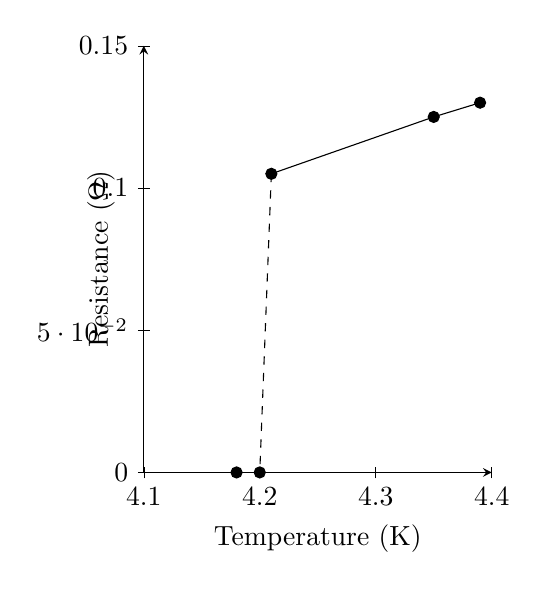
\begin{tikzpicture}
	\begin{axis}[
			width=6cm,
			height=7cm,
			xlabel={Temperature (K)},
			ylabel={Resistance ($\Omega$)},
			y label style = {at={(axis description cs:-0.055555,.5)},anchor=south},
			xmin=4.1,
			xmax=4.4,
			ymin=0,
			ymax=0.15,
			axis lines=left,
			tick style={black},
			no markers,
			samples=5
		]
		% Data points
		\addplot[only marks, mark=*] coordinates {
				(4.18, 0.000009)
				(4.20, 0.00001)
				(4.21, 0.105)
				(4.35, 0.125)
				(4.39, 0.130)
			};

		% Interpolation line
		\addplot[mark=*] coordinates {
				(4.21, 0.105)
				(4.35, 0.125)
				(4.39, 0.130)
			};

		\addplot[dashed, mark=*] coordinates {
				(4.21, 0.105)
				(4.20, 0.00001)
			};
	\end{axis}
\end{tikzpicture}

	\caption{The resistance of Mercury in function of the temperature of the sample, taken from~\cite{tsukerman2020compendium}}
	\label{img:mercury-resistance}
\end{figure}

Later studies discovered that many materials, pure and alloy, could be brought to the
superconducting state as long as three conditions were met:
\begin{itemize}
	\item The temperature of the sample didn't exceed the critical temperature $\tc$,
	\item The current density flowing in the sample didn't exceed the critical current
	      density $\jc$,
	\item The magnetic field acting on the material didn't exceed the critical magnetic field $\bc$.
\end{itemize}

When a material reaches the superconducting state it exhibits perfect diamagnetism, which means that
the material is able to perfectly expel the magnetic field lines from its volume (a simple experimental proof of this effect
is given by the magnetic levitation effect). This capacity was first observed by
Meissner and Ochsenfeld in 1933~\cite{meissner1933}. In 1935 the London's equations tried to explain
exotic behavior of different superconductor alloys which, in some situations, do not exhibit a perfectly diamagnetic behavior and allow the
penetration of external magnetic field lines down to a certain depth, known as the London's
penetration depth~\cite{london1935}. This property of superconductors was actually already theorized by Dutch
physicist Geertruida de Haas-Lorentz, who published some preliminary research in~\cite{fokker1925physica}.

The diamagnetic properties of superconductors depend heavily on the material microscopic properties. Two different Types of superconductors have been
identified and studied~\footnote{
	In general superconductor behavior can be explained through
	Ginzburg-Landau theory~\cite{Cyrot1973} but very recent research has proven that not every
	superconductor can be described using the \textsc{gl} equation as shown
	in~\cite{diamantini2023typeiiisuperconductivity}, this lead to the preliminary definition of
	a new type of superconductor, but, due to how recent the research is, it seems that, at the
	time of writing, nobody other than Diamantini published in the field of Type III superconductivity.
}, in the following I will provide a brief description of each.

\section{Type I superconductors}
\label{sec:type1}
\Cref{img:type1-transition}, plots magnetization, measuring the amount of induced or
permanent magnetic dipole moment of a magnet per unit volume~\cite{polarization-magnetization},
against external magnetic field $B$, applied on the sample. Once the magnetic field reaches $\bc$ the
magnetization of Type I superconductors drops to $0$.
\begin{figure}[!ht]
	\centering
	\begin{tikzpicture}
	% Axes
	\draw[->] (0,0) -- (5,0) node[right] {Applied Magnetic Fields, $B$};
	\draw[->] (0,0) -- (0,4) node[above] {Magnetization, $-M$};

	% Critical field B_c
	\node[below] at (3,0) {$B_c$};

	% Plot lines
	\draw[thick] (0,0) -- (3,3) -- (3,0);
\end{tikzpicture}

	\caption{Magnetization of a superconducting coil plotted against the external magnetic
		field, reproduction of the original plot taken from~\cite{slimani2022superconducting}}
\end{figure}
As long as the applied magnetic field is less than $\bc$, Type I superconductors exhibit perfect
diamagnetism, but once the material undergoes a transition to the normal-conducting
state (which will be referred to as \emph{quench} from now on) the magnetic dipole exerted by the
superconductor falls to zero (or a negligible value) allowing magnetic field penetration and making
such materials unsuitable for environments where a high magnetic field is required, such as fusion
reactors or particle physics experiments.

\section{Type II superconductors}
\label{sec:type2}
Type II superconductors, in most cases, are metal alloys. The characteristical impurity gives Type II superconductors an edge
over Type I, for high-field applications, due to the graceful degradation of magnetization with the increase in applied magnetic
field. A plot similar to \Cref{img:type1-transition} can be seen in \Cref{img:type2-transition}.
\begin{figure}[!ht]
	\centering
	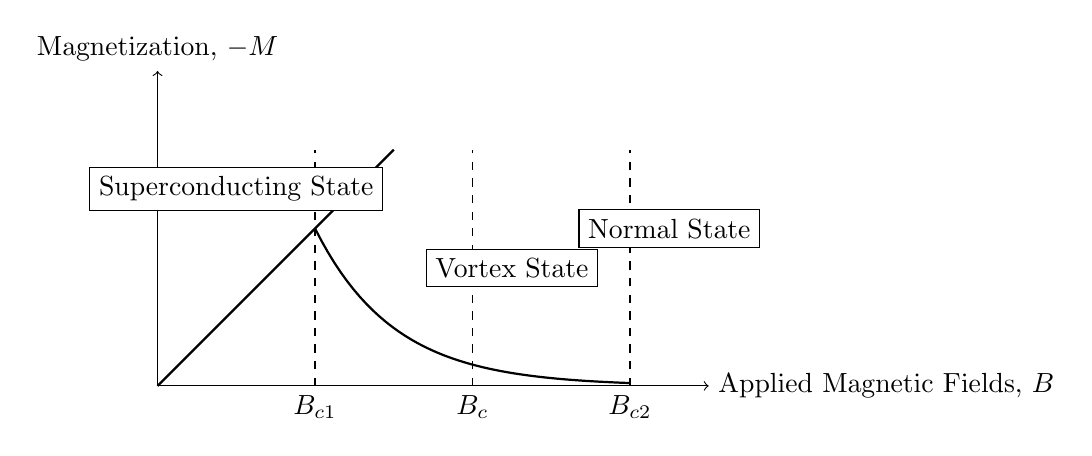
\begin{tikzpicture}
	% Axes
	\draw[->] (0,0) -- (7,0) node[right] {Applied Magnetic Fields, $B$};
	\draw[->] (0,0) -- (0,4) node[above] {Magnetization, $-M$};

	% Critical field labels
	\node[below] at (2,0) {$B_{c1}$};
	\node[below] at (4,0) {$B_c$};
	\node[below] at (6,0) {$B_{c2}$};

	% Dashed lines for critical fields
	\draw[dashed] (2,0) -- (2,3);
	\draw[dashed] (4,0) -- (4,3);
	\draw[dashed] (6,0) -- (6,3);

	% Magnetization curve
	\draw[thick] (0,0) -- (3,3);
	\draw[thick, domain=2:6, samples=50] plot (\x, {2*exp(-(\x-2))});

	% State labels with rectangles
	\node[draw, fill=white] at (1,2.5) {Superconducting State};
	\node[draw, fill=white] at (4.5,1.5) {Vortex State};
	\node[draw, fill=white] at (6.5,2) {Normal State};

\end{tikzpicture}

	\caption{Magnetization of a type II superconducting coil plotted against the external
		magnetic field, reproduction of the original plot taken from~\cite{slimani2022superconducting}}
	\label{img:type2-transition}
\end{figure}

Type II superconductors, while the applied magnetic field is less than $B_{C1}$, have the same
diamagnetic properties of Type I superconductors. Once the applied magnetic field surpasses the
$B_{C1}$ threshold, instead of having a very sharp transition from the superconducting state to
the normal-conducting state, these materials remain in an intermediate state referred to as the \emph{vortex} or \emph{hybrid state}.

In the vortex state the external magnetic field is partially penetrating in the volume of the superconductor, but the
flux lines are constrained in particular columns, pinned within the lattice of the
superconductor, called \emph{Abrikosov vortices} or \emph{fluxons}~\cite{abrikosov-vortices}.
A vortex is a closed-loop supercurrent surrounding the magnetic field lines that
penetrate the material. Supercurrents, also known as persistent currents, are extremely stable and as long as the material remains in the
superconducting state they don't decay~\cite{fujita-theory-HTS, file1963}, as a matter of fact, as long as the
fluxons are pinned in place, the material remains locally superconductive. Vortices are usually anchored to imperfections in the material, that is why alloys and anisotropic materials are usually Type II superconductors.

\begin{figure}[!ht]
	\centering
	\begin{tikzpicture}

	\pgfmathsetmacro{\z}{3}

	\foreach \x in {2, 4.5, 7} {
			\node (vortex) [cylinder, shape border rotate=90, draw,minimum height=3cm,
				minimum width=0.5cm] at (\x, 2, \z){};
			\draw[thick, ->] (\x,2,\z) -- (\x,4,\z) node[right] {};

			\foreach \y in {1, 2, 3} {
					\begin{scope}[shift={(\x,\y,\z)}]  % Shift the ellipse to (2,2) in XY plane
						\draw[thick, postaction={decorate}, decoration={markings, mark=at position 0.6 with {\arrow{>}}}] (0,0) ellipse (0.5 and 0.2);
					\end{scope}
				}
		}

	\draw[thick, ->] (10, 1, 3) -- (10, 4, 3) node[right] {$\mathbf{B}$};

	% Vertices of the cube
	\coordinate (A) at (0,0,0);
	\coordinate (B) at (8,0,0);
	\coordinate (C) at (8,3,0);
	\coordinate (D) at (0,3,0);
	\coordinate (E) at (0,0,3);
	\coordinate (F) at (8,0,3);
	\coordinate (G) at (8,3,3);
	\coordinate (H) at (0,3,3);

	% Draw the edges of the cube
	\draw
	(B) -- (C)
	(C) -- (D);
	\draw
	(E) -- (F) -- (G) -- (H) -- cycle;  % Top face
	\draw[dashed]
	(A) -- (B)
	(A) -- (E)
	(A) -- (D);
	\draw
	(B) -- (F)
	(C) -- (G)
	(D) -- (H);
\end{tikzpicture}

	\caption{Schematization of a lattice of vortices, each surrounded by a
		supercurrent.}
	\label{fig:abrikosov-lattice}
\end{figure}

\Cref{fig:abrikosov-lattice} is a simplified schema of the fluxon lattice, as we can see each
supercurrent (the rings in figure), surrounds a \emph{quantized} amount of magnetic flux
$\vec{\varphi}_0$. If a density of current $\vec{J}$ is flowing through a superconductor it will
generate a Lorentz force $\vec{F}_L = \vec{J} \times \vec{\varphi}_0$, capable of inducing vortex
movement, if the $\vec{J}$ is high enough. If the vortices begin to move under this influence, and
the generated electric field $\vec{E}$ is parallel to the direction of the current, then the motion
produces a dissipation of power due to Joule effect.

This was a simplified description of the effects of vortex movement in a superconductor lattice, not
taking into account many factors like flux pinning and quantum effects, for a more thorough
dissertation refer to~\cite{huebener2019}.

\section{Quench}
As was said in a previous section, whenever a superconductor exhibits a local transition to the
normal-conducting state, therefore developing a finite electrical resistance, an exponentially
growing cascade effect might occur. The transition might be particularly destructive if left
unchecked, because the presence of electrical resistance in a superconductor carrying a very high
current density might cause local joule heating power distribution that can lead to localized
material damage. That is why, normally, in the field of accelerator physics, superconducting magnets
are accompanied by \textsc{qps} (Quench Protection Systems), which interrupt power delivery whenever
one of the superconducting coils show an irreversible transition as a local rising of resistive
voltage in the electrical powering circuit.
